%% ODER: format ==         = "\mathrel{==}"
%% ODER: format /=         = "\neq "
%
%
\makeatletter
\@ifundefined{lhs2tex.lhs2tex.sty.read}%
  {\@namedef{lhs2tex.lhs2tex.sty.read}{}%
   \newcommand\SkipToFmtEnd{}%
   \newcommand\EndFmtInput{}%
   \long\def\SkipToFmtEnd#1\EndFmtInput{}%
  }\SkipToFmtEnd

\newcommand\ReadOnlyOnce[1]{\@ifundefined{#1}{\@namedef{#1}{}}\SkipToFmtEnd}
\usepackage{amstext}
\usepackage{amssymb}
\usepackage{stmaryrd}
\DeclareFontFamily{OT1}{cmtex}{}
\DeclareFontShape{OT1}{cmtex}{m}{n}
  {<5><6><7><8>cmtex8
   <9>cmtex9
   <10><10.95><12><14.4><17.28><20.74><24.88>cmtex10}{}
\DeclareFontShape{OT1}{cmtex}{m}{it}
  {<-> ssub * cmtt/m/it}{}
\newcommand{\texfamily}{\fontfamily{cmtex}\selectfont}
\DeclareFontShape{OT1}{cmtt}{bx}{n}
  {<5><6><7><8>cmtt8
   <9>cmbtt9
   <10><10.95><12><14.4><17.28><20.74><24.88>cmbtt10}{}
\DeclareFontShape{OT1}{cmtex}{bx}{n}
  {<-> ssub * cmtt/bx/n}{}
\newcommand{\tex}[1]{\text{\texfamily#1}}	% NEU

\newcommand{\Sp}{\hskip.33334em\relax}


\newcommand{\Conid}[1]{\mathit{#1}}
\newcommand{\Varid}[1]{\mathit{#1}}
\newcommand{\anonymous}{\kern0.06em \vbox{\hrule\@width.5em}}
\newcommand{\plus}{\mathbin{+\!\!\!+}}
\newcommand{\bind}{\mathbin{>\!\!\!>\mkern-6.7mu=}}
\newcommand{\rbind}{\mathbin{=\mkern-6.7mu<\!\!\!<}}% suggested by Neil Mitchell
\newcommand{\sequ}{\mathbin{>\!\!\!>}}
\renewcommand{\leq}{\leqslant}
\renewcommand{\geq}{\geqslant}
\usepackage{polytable}

%mathindent has to be defined
\@ifundefined{mathindent}%
  {\newdimen\mathindent\mathindent\leftmargini}%
  {}%

\def\resethooks{%
  \global\let\SaveRestoreHook\empty
  \global\let\ColumnHook\empty}
\newcommand*{\savecolumns}[1][default]%
  {\g@addto@macro\SaveRestoreHook{\savecolumns[#1]}}
\newcommand*{\restorecolumns}[1][default]%
  {\g@addto@macro\SaveRestoreHook{\restorecolumns[#1]}}
\newcommand*{\aligncolumn}[2]%
  {\g@addto@macro\ColumnHook{\column{#1}{#2}}}

\resethooks

\newcommand{\onelinecommentchars}{\quad-{}- }
\newcommand{\commentbeginchars}{\enskip\{-}
\newcommand{\commentendchars}{-\}\enskip}

\newcommand{\visiblecomments}{%
  \let\onelinecomment=\onelinecommentchars
  \let\commentbegin=\commentbeginchars
  \let\commentend=\commentendchars}

\newcommand{\invisiblecomments}{%
  \let\onelinecomment=\empty
  \let\commentbegin=\empty
  \let\commentend=\empty}

\visiblecomments

\newlength{\blanklineskip}
\setlength{\blanklineskip}{0.66084ex}

\newcommand{\hsindent}[1]{\quad}% default is fixed indentation
\let\hspre\empty
\let\hspost\empty
\newcommand{\NB}{\textbf{NB}}
\newcommand{\Todo}[1]{$\langle$\textbf{To do:}~#1$\rangle$}

\EndFmtInput
\makeatother
%
%
%
%
%
%
% This package provides two environments suitable to take the place
% of hscode, called "plainhscode" and "arrayhscode". 
%
% The plain environment surrounds each code block by vertical space,
% and it uses \abovedisplayskip and \belowdisplayskip to get spacing
% similar to formulas. Note that if these dimensions are changed,
% the spacing around displayed math formulas changes as well.
% All code is indented using \leftskip.
%
% Changed 19.08.2004 to reflect changes in colorcode. Should work with
% CodeGroup.sty.
%
\ReadOnlyOnce{polycode.fmt}%
\makeatletter

\newcommand{\hsnewpar}[1]%
  {{\parskip=0pt\parindent=0pt\par\vskip #1\noindent}}

% can be used, for instance, to redefine the code size, by setting the
% command to \small or something alike
\newcommand{\hscodestyle}{}

% The command \sethscode can be used to switch the code formatting
% behaviour by mapping the hscode environment in the subst directive
% to a new LaTeX environment.

\newcommand{\sethscode}[1]%
  {\expandafter\let\expandafter\hscode\csname #1\endcsname
   \expandafter\let\expandafter\endhscode\csname end#1\endcsname}

% "compatibility" mode restores the non-polycode.fmt layout.

\newenvironment{compathscode}%
  {\par\noindent
   \advance\leftskip\mathindent
   \hscodestyle
   \let\\=\@normalcr
   \let\hspre\(\let\hspost\)%
   \pboxed}%
  {\endpboxed\)%
   \par\noindent
   \ignorespacesafterend}

\newcommand{\compaths}{\sethscode{compathscode}}

% "plain" mode is the proposed default.
% It should now work with \centering.
% This required some changes. The old version
% is still available for reference as oldplainhscode.

\newenvironment{plainhscode}%
  {\hsnewpar\abovedisplayskip
   \advance\leftskip\mathindent
   \hscodestyle
   \let\hspre\(\let\hspost\)%
   \pboxed}%
  {\endpboxed%
   \hsnewpar\belowdisplayskip
   \ignorespacesafterend}

\newenvironment{oldplainhscode}%
  {\hsnewpar\abovedisplayskip
   \advance\leftskip\mathindent
   \hscodestyle
   \let\\=\@normalcr
   \(\pboxed}%
  {\endpboxed\)%
   \hsnewpar\belowdisplayskip
   \ignorespacesafterend}

% Here, we make plainhscode the default environment.

\newcommand{\plainhs}{\sethscode{plainhscode}}
\newcommand{\oldplainhs}{\sethscode{oldplainhscode}}
\plainhs

% The arrayhscode is like plain, but makes use of polytable's
% parray environment which disallows page breaks in code blocks.

\newenvironment{arrayhscode}%
  {\hsnewpar\abovedisplayskip
   \advance\leftskip\mathindent
   \hscodestyle
   \let\\=\@normalcr
   \(\parray}%
  {\endparray\)%
   \hsnewpar\belowdisplayskip
   \ignorespacesafterend}

\newcommand{\arrayhs}{\sethscode{arrayhscode}}

% The mathhscode environment also makes use of polytable's parray 
% environment. It is supposed to be used only inside math mode 
% (I used it to typeset the type rules in my thesis).

\newenvironment{mathhscode}%
  {\parray}{\endparray}

\newcommand{\mathhs}{\sethscode{mathhscode}}

% texths is similar to mathhs, but works in text mode.

\newenvironment{texthscode}%
  {\(\parray}{\endparray\)}

\newcommand{\texths}{\sethscode{texthscode}}

% The framed environment places code in a framed box.

\def\codeframewidth{\arrayrulewidth}
\RequirePackage{calc}

\newenvironment{framedhscode}%
  {\parskip=\abovedisplayskip\par\noindent
   \hscodestyle
   \arrayrulewidth=\codeframewidth
   \tabular{@{}|p{\linewidth-2\arraycolsep-2\arrayrulewidth-2pt}|@{}}%
   \hline\framedhslinecorrect\\{-1.5ex}%
   \let\endoflinesave=\\
   \let\\=\@normalcr
   \(\pboxed}%
  {\endpboxed\)%
   \framedhslinecorrect\endoflinesave{.5ex}\hline
   \endtabular
   \parskip=\belowdisplayskip\par\noindent
   \ignorespacesafterend}

\newcommand{\framedhslinecorrect}[2]%
  {#1[#2]}

\newcommand{\framedhs}{\sethscode{framedhscode}}

% The inlinehscode environment is an experimental environment
% that can be used to typeset displayed code inline.

\newenvironment{inlinehscode}%
  {\(\def\column##1##2{}%
   \let\>\undefined\let\<\undefined\let\\\undefined
   \newcommand\>[1][]{}\newcommand\<[1][]{}\newcommand\\[1][]{}%
   \def\fromto##1##2##3{##3}%
   \def\nextline{}}{\) }%

\newcommand{\inlinehs}{\sethscode{inlinehscode}}

% The joincode environment is a separate environment that
% can be used to surround and thereby connect multiple code
% blocks.

\newenvironment{joincode}%
  {\let\orighscode=\hscode
   \let\origendhscode=\endhscode
   \def\endhscode{\def\hscode{\endgroup\def\@currenvir{hscode}\\}\begingroup}
   %\let\SaveRestoreHook=\empty
   %\let\ColumnHook=\empty
   %\let\resethooks=\empty
   \orighscode\def\hscode{\endgroup\def\@currenvir{hscode}}}%
  {\origendhscode
   \global\let\hscode=\orighscode
   \global\let\endhscode=\origendhscode}%

\makeatother
\EndFmtInput
%

\section{Implementation in Haskell}
In this section, we present (some fragments of) an implementation of
\cref{ch4:pmfdclass} in
\emph{Haskell}.\footnote{\href{http://www.haskell.org/}{\url{www.haskell.org}}}
In the printed copies of this thesis, the complete software is included
on a CD at the end of this thesis, and in the near future the code can also be
found on the author's github
page.\footnote{\href{https://github.com/J0J0/}{\url{www.github.com/J0J0}}%
\;\;(J-zero-J-zero)}
See \cref{ch4:tab:funcs1} at the end of the section for a correspondence between
the presented types/functions and the modules they are defined in.

Our basic types are \ensuremath{\Conid{Vertex}}, \ensuremath{\Conid{Simplex}} and \ensuremath{\Conid{Complex}} that are defined as
follows:
\begin{hscode}\SaveRestoreHook
\column{B}{@{}>{\hspre}l<{\hspost}@{}}%
\column{E}{@{}>{\hspre}l<{\hspost}@{}}%
\>[B]{}\mathbf{data}\;\Conid{Vertex}\;\Varid{a}\;\mathbf{where}\;\Conid{Vertex}\mathbin{::}(\Conid{Eq}\;\Varid{a})\Rightarrow \Varid{a}\to \Conid{Vertex}\;\Varid{a}{}\<[E]%
\\[\blanklineskip]%
\>[B]{}\mathbf{type}\;\Conid{Simplex}\;\Varid{a}\mathrel{=}[\mskip1.5mu \Conid{Vertex}\;\Varid{a}\mskip1.5mu]{}\<[E]%
\\[\blanklineskip]%
\>[B]{}\mathbf{type}\;\Conid{Complex}\;\Varid{a}\mathrel{=}[\mskip1.5mu \Conid{Simplex}\;\Varid{a}\mskip1.5mu]{}\<[E]%
\ColumnHook
\end{hscode}\resethooks
A \ensuremath{\Conid{Vertex}} can be basically anything, but we require an \ensuremath{\Conid{Eq}} context
(which should not be much of a restriction). (Note, that this declaration
uses a GADT\footnote{generalised algebraic datatype,
\href{http://www.haskell.org/haskellwiki/Generalised_algebraic_datatype}{%
\url{www.haskell.org/haskellwiki/Generalised_algebraic_datatype}}}
to enforce that vertices can be tested for equality.) A \enquote{set}
of vertices is a list in Haskell and likewise for complexes. Of course,
this allows \enquote{simplices with repeated vertices} or similar anomalies,
so it is the programer's job to make sure that such (invalid) complexes
are not passed to the library.

Let $K$ be a finite weak $2$-pseudomanifold. To identify the closed
surfaces~$S_j$ such that $\geom{K} \cong (\coprod_{j=1}^k S_j)/{\sim}$ 
(which exist by \cref{ch4:pmfdclass}) we proceed as follows:
The proof of \cref{ch4:pmfdclass} and the preceding proposition provide us with an
algorithm for identifying a vertex as a singularity and for resolving the
latter. We test each vertex, fix the singularity if necessary and finally
obtain a complex~$K'$ such that $\geom{K'}$ is a compact $2$-manifold. Then
we isolate the connected components of~$K'$ and for each component~$L\subset K'$
we identify the surface~$\geom{L}$. If we are only interested in the closed
surfaces~$S_j$, we are done here, but if we also want to specify how they
are glued together, further examination of~$K'$ is required.

We get back to the gluing problem later and start with the identification
of the surfaces~$S_j$. Assume that $K$ is given as \ensuremath{\Varid{c}\mathbin{::}\Conid{Complex}\;\Varid{a}} and
that \ensuremath{\Varid{v}\mathbin{::}\Conid{Vertex}\;\Varid{a}} is a vertex of \ensuremath{\Varid{c}}. Then \ensuremath{\Varid{fixSingularity}\;\Varid{v}\;\Varid{c}} returns
a complex with the singularity at (the vertex corresponding to) \ensuremath{\Varid{v}} resolved.
Here is the corresponding code:
\begin{hscode}\SaveRestoreHook
\column{B}{@{}>{\hspre}l<{\hspost}@{}}%
\column{5}{@{}>{\hspre}l<{\hspost}@{}}%
\column{9}{@{}>{\hspre}l<{\hspost}@{}}%
\column{10}{@{}>{\hspre}l<{\hspost}@{}}%
\column{14}{@{}>{\hspre}c<{\hspost}@{}}%
\column{14E}{@{}l@{}}%
\column{15}{@{}>{\hspre}c<{\hspost}@{}}%
\column{15E}{@{}l@{}}%
\column{17}{@{}>{\hspre}l<{\hspost}@{}}%
\column{18}{@{}>{\hspre}l<{\hspost}@{}}%
\column{19}{@{}>{\hspre}l<{\hspost}@{}}%
\column{22}{@{}>{\hspre}l<{\hspost}@{}}%
\column{23}{@{}>{\hspre}l<{\hspost}@{}}%
\column{24}{@{}>{\hspre}c<{\hspost}@{}}%
\column{24E}{@{}l@{}}%
\column{27}{@{}>{\hspre}l<{\hspost}@{}}%
\column{E}{@{}>{\hspre}l<{\hspost}@{}}%
\>[B]{}\Varid{fixSingularity}\mathbin{::}(\Conid{Eq}\;\Varid{a})\Rightarrow \Conid{Vertex}\;\Varid{a}\to \Conid{Complex}\;\Varid{a}\to \Conid{Complex}\;(\Varid{a},\Conid{Int}){}\<[E]%
\\
\>[B]{}\Varid{fixSingularity}\;\Varid{v}\;\Varid{c}\mathrel{=}{}\<[E]%
\\
\>[B]{}\hsindent{5}{}\<[5]%
\>[5]{}\mathbf{let}\;{}\<[10]%
\>[10]{}\Varid{f}{}\<[14]%
\>[14]{}\mathrel{=}{}\<[14E]%
\>[17]{}\Varid{id}\mathbin{\&\&\&}\Varid{const}\;\mathrm{0}{}\<[E]%
\\
\>[10]{}\Varid{c'}{}\<[14]%
\>[14]{}\mathrel{=}{}\<[14E]%
\>[17]{}\Varid{complexMap}\;\Varid{f}\;\Varid{c}{}\<[E]%
\\
\>[10]{}\Varid{v'}{}\<[14]%
\>[14]{}\mathrel{=}{}\<[14E]%
\>[17]{}\Varid{vMap}\;\Varid{f}\;\Varid{v}{}\<[E]%
\\
\>[B]{}\hsindent{5}{}\<[5]%
\>[5]{}\mathbf{in}\;{}\<[9]%
\>[9]{}\Varid{fixSingularity'}\;\Varid{v'}\;\Varid{c'}{}\<[E]%
\\[\blanklineskip]%
\>[B]{}\Varid{fixSingularity'}\mathbin{::}(\Conid{Eq}\;\Varid{a})\Rightarrow \Conid{Vertex}\;(\Varid{a},\Conid{Int})\to \Conid{Complex}\;(\Varid{a},\Conid{Int})\to \Conid{Complex}\;(\Varid{a},\Conid{Int}){}\<[E]%
\\
\>[B]{}\Varid{fixSingularity'}\;\Varid{v}\;\Varid{c}\mathrel{=}{}\<[E]%
\\
\>[B]{}\hsindent{5}{}\<[5]%
\>[5]{}\mathbf{case}\;\Varid{starSummands}\;\Varid{v}\;\Varid{c}\;\mathbf{of}{}\<[E]%
\\
\>[5]{}\hsindent{4}{}\<[9]%
\>[9]{}\anonymous \mathbin{:}[\mskip1.5mu \mskip1.5mu]{}\<[15]%
\>[15]{}\to {}\<[15E]%
\>[19]{}\Varid{c}{}\<[E]%
\\
\>[5]{}\hsindent{4}{}\<[9]%
\>[9]{}\Varid{sSs}{}\<[15]%
\>[15]{}\to {}\<[15E]%
\>[19]{}\Varid{fixSingularity''}\;\Varid{v}\;\Varid{sSs}\;\Varid{c}{}\<[E]%
\\[\blanklineskip]%
\>[B]{}\Varid{fixSingularity''}\mathbin{::}\mbox{\small(type omitted)}{}\<[E]%
\\
\>[B]{}\Varid{fixSingularity''}\;\Varid{v}\;\Varid{sSs}\;\Varid{c}\mathrel{=}{}\<[E]%
\\
\>[B]{}\hsindent{5}{}\<[5]%
\>[5]{}\mathbf{let}\;{}\<[10]%
\>[10]{}\Varid{sSs'}\mathrel{=}\Varid{map}\;(\Varid{parentSimplices}\;[\mskip1.5mu \Varid{v}\mskip1.5mu]\mathbin{\circ}\Varid{generatedBy})\;\Varid{sSs}{}\<[E]%
\\
\>[10]{}\Varid{oldSimplices}{}\<[24]%
\>[24]{}\mathrel{=}{}\<[24E]%
\>[27]{}[\mskip1.5mu \Varid{v}\mskip1.5mu]\mathbin{:}\Varid{concatMap}\;(\Varid{delete}\;[\mskip1.5mu \Varid{v}\mskip1.5mu])\;\Varid{sSs'}{}\<[E]%
\\
\>[10]{}\Varid{newSimplices}{}\<[24]%
\>[24]{}\mathrel{=}{}\<[24E]%
\>[27]{}\Varid{concatMap}\;(\Varid{replaceStarSummand}\;\Varid{v})\mathbin{\$}[\mskip1.5mu \mathrm{1}\mathinner{\ldotp\ldotp}\mskip1.5mu]\mathbin{`\Varid{zip}`}\Varid{sSs'}{}\<[E]%
\\
\>[B]{}\hsindent{5}{}\<[5]%
\>[5]{}\mathbf{in}\;{}\<[9]%
\>[9]{}(\Varid{c}\mathbin{\char92 \char92 }\Varid{oldSimplices})\mathbin{`\Varid{union}`}\Varid{newSimplices}{}\<[E]%
\\[\blanklineskip]%
\>[B]{}\\[-1.2\baselineskip]{}\<[E]%
\\[\blanklineskip]%
\>[B]{}\Varid{starSummands}\mathbin{::}\Conid{Vertex}\;\Varid{a}\to \Conid{Complex}\;\Varid{a}\to \Conid{StarSummands}\;\Varid{a}{}\<[E]%
\\
\>[B]{}\Varid{starSummands}\mathrel{=}\Varid{findSummands}\mathbin{.:}\Varid{star}{}\<[E]%
\\[\blanklineskip]%
\>[B]{}\Varid{findSummands}\mathbin{::}\Conid{Complex}\;\Varid{a}\to \Conid{StarSummands}\;\Varid{a}{}\<[E]%
\\
\>[B]{}\Varid{findSummands}\;\Varid{st}\mathrel{=}{}\<[E]%
\\
\>[B]{}\hsindent{5}{}\<[5]%
\>[5]{}\mathbf{case}\;\Varid{filter}\;(\Varid{isNSimplex}\;\mathrm{2})\;\Varid{st}\;\mathbf{of}{}\<[E]%
\\
\>[5]{}\hsindent{4}{}\<[9]%
\>[9]{}[\mskip1.5mu \mskip1.5mu]{}\<[14]%
\>[14]{}\to {}\<[14E]%
\>[18]{}[\mskip1.5mu \mskip1.5mu]{}\<[E]%
\\
\>[5]{}\hsindent{4}{}\<[9]%
\>[9]{}\Varid{s}\mathbin{:\char95 }{}\<[14]%
\>[14]{}\to {}\<[14E]%
\>[18]{}\mathbf{let}\;{}\<[23]%
\>[23]{}\Varid{summand}\mathrel{=}\Varid{dfsSimplices}\;\Varid{st}\;\Varid{s}{}\<[E]%
\\
\>[23]{}\Varid{st'}\mathrel{=}\Varid{st}\mathbin{\char92 \char92 }\Varid{summand}{}\<[E]%
\\
\>[18]{}\mathbf{in}\;{}\<[22]%
\>[22]{}\Varid{summand}\mathbin{:}\Varid{findSummands}\;\Varid{st'}{}\<[E]%
\ColumnHook
\end{hscode}\resethooks
To be able to split a vertex into multiple copies (like in the proof of
\cref{ch4:pmfdclass}), we first transform \ensuremath{\Varid{c}} into \ensuremath{\Varid{c'}\mathbin{::}\Conid{Complex}\;(\Varid{a},\Conid{Int})}
where each vertex has the index~$0$ attached. The function \ensuremath{\Varid{fixSingularity'}}
obtains the wedge summands of $\st(v)$ and passes them to \ensuremath{\Varid{fixSingularity''}}
unless there is no singularity at~\ensuremath{\Varid{v}}. The latter function then implements
what is described in the proof of the theorem (where \ensuremath{\Varid{parentSimplices}\;\Varid{s}\;\Varid{c1}}
returns all simplices of $c_1$ of which \ensuremath{\Varid{s}} is a face).
The computation of the star summands are quite clear once we explain what
\ensuremath{\Varid{dfsSimplices}} does. \emph{Dfs} is an abbreviation for \emph{depth first
search}, a common algorithm for graph traversal. In this case
\ensuremath{\Varid{dfsSimplices}\;\Varid{c1}\;\Varid{s1}} starts at a simplex $s_1\in c_1$ of dimension~$d$ and
returns all $d$-simplices of~$c_1$ that share a common $(d{-}1)$-dimensional face
with~$s_1$ or another simplex already visited. For instance, \ensuremath{\Varid{dfsSimplices}\;\Varid{c}\;\Varid{s}}
for any $2$-simplex~\ensuremath{\Varid{s}} of~\ensuremath{\Varid{c}} returns all $2$-simplices of~\ensuremath{\Varid{c}} if and only if
\ensuremath{\Varid{c}} is strongly connected.

Now assume that we resolved all singularities and that we already called\begin{hscode}\SaveRestoreHook
\column{B}{@{}>{\hspre}l<{\hspost}@{}}%
\column{3}{@{}>{\hspre}l<{\hspost}@{}}%
\column{E}{@{}>{\hspre}l<{\hspost}@{}}%
\>[3]{}\Varid{connectedComponents}\mathbin{::}\Conid{Complex}\;\Varid{a}\to [\mskip1.5mu \Conid{Complex}\;\Varid{a}\mskip1.5mu]{}\<[E]%
\ColumnHook
\end{hscode}\resethooks
on the resulting complex. Thus we are left with the task to identify a surface
complex. This is done by the function \ensuremath{\Varid{identifySurface}} which takes a complex
and has the following return type:
\begin{hscode}\SaveRestoreHook
\column{B}{@{}>{\hspre}l<{\hspost}@{}}%
\column{28}{@{}>{\hspre}l<{\hspost}@{}}%
\column{42}{@{}>{\hspre}c<{\hspost}@{}}%
\column{42E}{@{}l@{}}%
\column{46}{@{}>{\hspre}l<{\hspost}@{}}%
\column{55}{@{}>{\hspre}l<{\hspost}@{}}%
\column{E}{@{}>{\hspre}l<{\hspost}@{}}%
\>[B]{}\mathbf{data}\;\Conid{Surface}\mathrel{=}\Conid{Surface}\;\{\mskip1.5mu {}\<[28]%
\>[28]{}\Varid{isOrientable}{}\<[42]%
\>[42]{}\mathbin{::}{}\<[42E]%
\>[46]{}\Conid{Bool},{}\<[E]%
\\
\>[28]{}\Varid{genus}{}\<[42]%
\>[42]{}\mathbin{::}{}\<[42E]%
\>[46]{}\Conid{Integer}{}\<[55]%
\>[55]{}\mskip1.5mu\}\;\mathbf{deriving}\;(\Conid{Eq},\Conid{Ord}){}\<[E]%
\ColumnHook
\end{hscode}\resethooks
(i.\,e. we uniquely identify a closed surface via orientability
and its genus). Instead of including the implementation of
\ensuremath{\Varid{identifySurface}} here, we only explain how it works. Basically,
there are two approaches that come to mind:
\begin{itemize}[topsep=5pt,labelindent=0pt]
\item
    Determine the orientability type explicitely and calculate the genus from
    the Euler characteristic.
\item
    Compute a \emph{fundamental polygon} of the complex and analyse
    the labelling scheme.
\end{itemize}
Our implementation follows the latter strategy since we need its functionality
in \cref{ch4:sec:loopspmfd} anyway. To be a little bit more specific, we do the
following: paste all $2$-simplices together to obtain a polygon with edges to be
identified in pairs; normalize the resulting labelling scheme; determine the
surface type from the normal form. The whole process, known as the
classification of closed surfaces, can be found in the topology book by
Munkres~\cite[Ch.~12]{bookc:munkres00}.

Put together, the above discussion becomes the desired identification of the
closed surfaces~$S_j$. The function
\begin{hscode}\SaveRestoreHook
\column{B}{@{}>{\hspre}l<{\hspost}@{}}%
\column{E}{@{}>{\hspre}l<{\hspost}@{}}%
\>[B]{}\Varid{baseSurfaces}\mathbin{::}(\Conid{Eq}\;\Varid{a})\Rightarrow \Conid{Complex}\;\Varid{a}\to [\mskip1.5mu \Conid{Surface}\mskip1.5mu]{}\<[E]%
\\
\>[B]{}\Varid{baseSurfaces}\mathrel{=}\Varid{map}\;\Varid{identifySurface}\mathbin{\circ}\Varid{connectedComponents}\mathbin{\circ}\Varid{fixAllSingularities}{}\<[E]%
\ColumnHook
\end{hscode}\resethooks
composes the functions we met before (or a slight variation in case of
\ensuremath{\Varid{fixAllSingularities}}). It takes a complex and yields a list of surfaces,
the~$S_j$ for the particular complex. For instance, assume that \ensuremath{\Varid{tor}} is a
complex that triangulates the torus, \ensuremath{\mathbin{\#}} denotes connected sum and \ensuremath{\mathbin{\char92 /}}
denotes wedge sum. Then we have:\begin{hscode}\SaveRestoreHook
\column{B}{@{}>{\hspre}l<{\hspost}@{}}%
\column{3}{@{}>{\hspre}l<{\hspost}@{}}%
\column{38}{@{}>{\hspre}l<{\hspost}@{}}%
\column{E}{@{}>{\hspre}l<{\hspost}@{}}%
\>[3]{}\Varid{baseSurfaces}\;\Varid{tor}{}\<[38]%
\>[38]{}\qquad\mbox{\onelinecomment   [OS.g=1]}{}\<[E]%
\\
\>[3]{}\Varid{baseSurfaces}\mathbin{\$}(\Varid{tor}\mathbin{\#}\Varid{tor})\mathbin{\char92 /}\Varid{tor}{}\<[38]%
\>[38]{}\qquad\mbox{\onelinecomment   [OS.g=2,OS.g=1]}{}\<[E]%
\ColumnHook
\end{hscode}\resethooks
where \enquote{OS.g=r} means \enquote{orientable surface of genus~$r$}.

Now we treat the gluing. Remeber that we have $\geom{K} \cong
(\coprod_{j=1}^k S_j)/{\sim}$ where $\sim$ is an equivalence relation that
identifies only finitely many points. Since the exact relation $\sim$ is
neither relevant nor convenient to work with, we strip the gluing information
down to a \emph{gluing graph}, determined by the following data:
\begin{itemize}[topsep=5pt,labelindent=0pt]
\item
    a set $N_{\mr g}$ of (abstract) gluing nodes,
\item
    the set $N_{\mr s} \defeq \{S_1,\dots,S_k\}$ of surface nodes,
\item
    and a function $e\colon N_{\mr g}\times N_{\mr s}\to\N$ that
    specifies how often a surface is glued to a particular
    gluing point.
\end{itemize}
Note that this defines a (bipartite) multigraph (whithout self-loops).
In our implementation we use the following types to store the multigraph
(where \ensuremath{\Conid{M}} and \ensuremath{\Conid{LM}} are \ensuremath{\Conid{\Conid{Data}.\Conid{Map}.Strict}} and .\ensuremath{\Conid{Lazy}}, respectively):
\begin{hscode}\SaveRestoreHook
\column{B}{@{}>{\hspre}l<{\hspost}@{}}%
\column{21}{@{}>{\hspre}l<{\hspost}@{}}%
\column{24}{@{}>{\hspre}l<{\hspost}@{}}%
\column{25}{@{}>{\hspre}c<{\hspost}@{}}%
\column{25E}{@{}l@{}}%
\column{26}{@{}>{\hspre}l<{\hspost}@{}}%
\column{28}{@{}>{\hspre}l<{\hspost}@{}}%
\column{39}{@{}>{\hspre}c<{\hspost}@{}}%
\column{39E}{@{}l@{}}%
\column{43}{@{}>{\hspre}l<{\hspost}@{}}%
\column{E}{@{}>{\hspre}l<{\hspost}@{}}%
\>[B]{}\mathbf{type}\;\Conid{GluingGraphD}{}\<[25]%
\>[25]{}\mathrel{=}{}\<[25E]%
\>[28]{}\Conid{\Conid{M}.Map}\;(\Conid{Int},\Conid{Int})\;\Conid{Int}{}\<[E]%
\\
\>[B]{}\mathbf{type}\;\Conid{GluedObj}\;\Varid{o}{}\<[25]%
\>[25]{}\mathrel{=}{}\<[25E]%
\>[28]{}\Conid{\Conid{LM}.Map}\;\Conid{Int}\;\Varid{o}{}\<[E]%
\\
\>[B]{}\mathbf{type}\;\Conid{GluedVertices}\;{}\<[21]%
\>[21]{}\Varid{a}{}\<[25]%
\>[25]{}\mathrel{=}{}\<[25E]%
\>[28]{}\Conid{GluedObj}\;(\Conid{Vertex}\;\Varid{a}){}\<[E]%
\\
\>[B]{}\mathbf{type}\;\Conid{GluedComplexes}\;\Varid{a}{}\<[25]%
\>[25]{}\mathrel{=}{}\<[25E]%
\>[28]{}\Conid{GluedObj}\;(\Conid{Complex}\;(\Varid{a},\Conid{Int})){}\<[E]%
\\
\>[B]{}\mathbf{data}\;\Conid{GluedD}\;\Varid{a}\mathrel{=}\Conid{GluedD}\;\{\mskip1.5mu {}\<[E]%
\\
\>[B]{}\hsindent{26}{}\<[26]%
\>[26]{}\Varid{glGraphD}{}\<[39]%
\>[39]{}\mathbin{::}{}\<[39E]%
\>[43]{}\Conid{GluingGraphD}{}\<[E]%
\\
\>[B]{}\hsindent{24}{}\<[24]%
\>[24]{},\Varid{glVertices}{}\<[39]%
\>[39]{}\mathbin{::}{}\<[39E]%
\>[43]{}\Conid{GluedVertices}\;\Varid{a}{}\<[E]%
\\
\>[B]{}\hsindent{24}{}\<[24]%
\>[24]{},\Varid{glComplexes}{}\<[39]%
\>[39]{}\mathbin{::}{}\<[39E]%
\>[43]{}\Conid{GluedComplexes}\;\Varid{a}\mskip1.5mu\}{}\<[E]%
\ColumnHook
\end{hscode}\resethooks
\ensuremath{\Conid{GluingGraphD}} represents $e$; a node (of either type) is an \ensuremath{\Conid{Int}} which is
mapped by \ensuremath{\Conid{GluedVertices}} and \ensuremath{\Conid{GluedComplexes}} to the corresponding object.
\ensuremath{\Conid{GlueD}} combines all gluing data that we work with.
To extract that data from the weak pseudomanifold, we use the next two functions
(with accompanying helpers):
\begin{hscode}\SaveRestoreHook
\column{B}{@{}>{\hspre}l<{\hspost}@{}}%
\column{5}{@{}>{\hspre}l<{\hspost}@{}}%
\column{9}{@{}>{\hspre}l<{\hspost}@{}}%
\column{13}{@{}>{\hspre}l<{\hspost}@{}}%
\column{20}{@{}>{\hspre}c<{\hspost}@{}}%
\column{20E}{@{}l@{}}%
\column{23}{@{}>{\hspre}l<{\hspost}@{}}%
\column{24}{@{}>{\hspre}c<{\hspost}@{}}%
\column{24E}{@{}l@{}}%
\column{27}{@{}>{\hspre}l<{\hspost}@{}}%
\column{E}{@{}>{\hspre}l<{\hspost}@{}}%
\>[B]{}\Varid{gluingGraph}\mathbin{::}(\Conid{Eq}\;\Varid{a})\Rightarrow \Conid{Complex}\;\Varid{a}\to \Conid{GluedD}\;\Varid{a}{}\<[E]%
\\
\>[B]{}\Varid{gluingGraph}\mathrel{=}\Varid{gluingGraphFromFixed}\mathbin{\circ}\Varid{fixAllSingularities}{}\<[E]%
\\[\blanklineskip]%
\>[B]{}\Varid{gluingGraphFromFixed}\mathbin{::}(\Conid{Eq}\;\Varid{a})\Rightarrow \Conid{Complex}\;(\Varid{a},\Conid{Int})\to \Conid{GluedD}\;\Varid{a}{}\<[E]%
\\
\>[B]{}\Varid{gluingGraphFromFixed}\;\Varid{c}\mathrel{=}{}\<[E]%
\\
\>[B]{}\hsindent{5}{}\<[5]%
\>[5]{}\Conid{GluedD}\;\{\mskip1.5mu \Varid{glGraphD}\mathrel{=}\Varid{graph},\;\Varid{glVertices}\mathrel{=}\Varid{vsm},\;\Varid{glComplexes}\mathrel{=}\Varid{comps}\mskip1.5mu\}{}\<[E]%
\\
\>[5]{}\hsindent{4}{}\<[9]%
\>[9]{}\mathbf{where}{}\<[E]%
\\
\>[9]{}\hsindent{4}{}\<[13]%
\>[13]{}\Varid{comps}{}\<[20]%
\>[20]{}\mathrel{=}{}\<[20E]%
\>[23]{}\Varid{\Conid{LM}.fromDistinctAscList}\mathbin{\$}[\mskip1.5mu \mathrm{0}\mathinner{\ldotp\ldotp}\mskip1.5mu]\mathbin{`\Varid{zip}`}\Varid{connectedComponents}\;\Varid{c}{}\<[E]%
\\
\>[9]{}\hsindent{4}{}\<[13]%
\>[13]{}\Varid{vs}{}\<[20]%
\>[20]{}\mathrel{=}{}\<[20E]%
\>[23]{}\Varid{nub}\mathbin{\$}\Varid{map}\;(\Varid{vMap}\;\Varid{fst})\mathbin{\$}\Varid{filter}\;\Varid{isGluedV}\mathbin{\$}\Varid{vertices}\;\Varid{c}{}\<[E]%
\\
\>[9]{}\hsindent{4}{}\<[13]%
\>[13]{}\Varid{vsi}{}\<[20]%
\>[20]{}\mathrel{=}{}\<[20E]%
\>[23]{}\Varid{vs}\mathbin{`\Varid{zip}`}[\mskip1.5mu \mathrm{0}\mathinner{\ldotp\ldotp}\mskip1.5mu]{}\<[E]%
\\
\>[9]{}\hsindent{4}{}\<[13]%
\>[13]{}\Varid{vsm}{}\<[20]%
\>[20]{}\mathrel{=}{}\<[20E]%
\>[23]{}\Varid{\Conid{LM}.fromDistinctAscList}\mathbin{\$}\Varid{map}\;\Varid{swap}\;\Varid{vsi}{}\<[E]%
\\
\>[9]{}\hsindent{4}{}\<[13]%
\>[13]{}\Varid{graph}{}\<[20]%
\>[20]{}\mathrel{=}{}\<[20E]%
\>[23]{}\Varid{\Conid{LM}.foldrWithKey}\;(\Varid{addGluingData}\;\Varid{vsi})\;\Varid{\Conid{M}.empty}\;\Varid{comps}{}\<[E]%
\\[\blanklineskip]%
\>[B]{}\Varid{isGluedV}\mathbin{::}\Conid{Vertex}\;(\Varid{a},\Conid{Int})\to \Conid{Bool}{}\<[E]%
\\
\>[B]{}\Varid{isGluedV}\;(\Conid{Vertex}\;(\anonymous ,\Varid{t}))\mathrel{=}\Varid{t}\not\equiv \mathrm{0}{}\<[E]%
\\[\blanklineskip]%
\>[B]{}\Varid{addGluingData}\mathbin{::}\mbox{\small(type omitted)}{}\<[E]%
\\
\>[B]{}\Varid{addGluingData}\;\Varid{vsi}\;\Varid{j}\;\Varid{comp}\;\Varid{m}\mathrel{=}{}\<[E]%
\\
\>[B]{}\hsindent{5}{}\<[5]%
\>[5]{}\Varid{foldr}\;(\lambda \Varid{v}\to \Varid{\Conid{M}.insertWith}\;(\mathbin{+})\;(\Varid{toId}\;\Varid{v},\Varid{j})\;\mathrm{1})\;\Varid{m}\;\Varid{gluedToVs}{}\<[E]%
\\
\>[5]{}\hsindent{4}{}\<[9]%
\>[9]{}\mathbf{where}{}\<[E]%
\\
\>[9]{}\hsindent{4}{}\<[13]%
\>[13]{}\Varid{gluedVs}{}\<[24]%
\>[24]{}\mathrel{=}{}\<[24E]%
\>[27]{}\Varid{filter}\;\Varid{isGluedV}\mathbin{\$}\Varid{vertices}\;\Varid{comp}{}\<[E]%
\\
\>[9]{}\hsindent{4}{}\<[13]%
\>[13]{}\Varid{gluedToVs}{}\<[24]%
\>[24]{}\mathrel{=}{}\<[24E]%
\>[27]{}\Varid{map}\;(\Varid{vMap}\;\Varid{fst})\;\Varid{gluedVs}{}\<[E]%
\\
\>[9]{}\hsindent{4}{}\<[13]%
\>[13]{}\Varid{toId}\;\Varid{v}{}\<[24]%
\>[24]{}\mathrel{=}{}\<[24E]%
\>[27]{}\Varid{fromJust}\mathbin{\$}\Varid{lookup}\;\Varid{v}\;\Varid{vsi}{}\<[E]%
\ColumnHook
\end{hscode}\resethooks
Furthermore, we provide a utility function that extracts the most interesting
parts from a \ensuremath{\Conid{GluedD}}, that is the actual multigraph (as a \ensuremath{\Conid{GluingGraphD}})
and the glued surfaces (identified as \ensuremath{\Conid{Surface}}):
\begin{hscode}\SaveRestoreHook
\column{B}{@{}>{\hspre}l<{\hspost}@{}}%
\column{21}{@{}>{\hspre}c<{\hspost}@{}}%
\column{21E}{@{}l@{}}%
\column{24}{@{}>{\hspre}l<{\hspost}@{}}%
\column{E}{@{}>{\hspre}l<{\hspost}@{}}%
\>[B]{}\mathbf{type}\;\Conid{GluedSurfaces}{}\<[21]%
\>[21]{}\mathrel{=}{}\<[21E]%
\>[24]{}\Conid{GluedObj}\;\Conid{Surface}{}\<[E]%
\\[\blanklineskip]%
\>[B]{}\Varid{gluingGraphSurf}\mathbin{::}(\Conid{Eq}\;\Varid{a})\Rightarrow \Conid{Complex}\;\Varid{a}\to (\Conid{GluingGraphD},\Conid{GluedSurfaces}){}\<[E]%
\\
\>[B]{}\Varid{gluingGraphSurf}\mathrel{=}(\Varid{glGraphD}\mathbin{\&\&\&}\Varid{identifyGluedSurfaces})\mathbin{\circ}\Varid{gluingGraph}{}\<[E]%
\\[\blanklineskip]%
\>[B]{}\Varid{identifyGluedSurfaces}\mathbin{::}\Conid{GluedD}\;\Varid{a}\to \Conid{GluedSurfaces}{}\<[E]%
\\
\>[B]{}\Varid{identifyGluedSurfaces}\mathrel{=}\Varid{\Conid{LM}.map}\;\Varid{identifySurface}\mathbin{\circ}\Varid{glComplexes}{}\<[E]%
\ColumnHook
\end{hscode}\resethooks
The functions\begin{hscode}\SaveRestoreHook
\column{B}{@{}>{\hspre}l<{\hspost}@{}}%
\column{3}{@{}>{\hspre}l<{\hspost}@{}}%
\column{E}{@{}>{\hspre}l<{\hspost}@{}}%
\>[3]{}\Varid{writeGluingGraph}\mathbin{::}(\Conid{GluingGraphD},\Conid{GluedSurfaces})\to \Conid{FilePath}\to \Conid{IO}\;(){}\<[E]%
\\
\>[3]{}\Varid{visualizeGluingGraph}\mathbin{::}(\Conid{GluingGraphD},\Conid{GluedSurfaces})\to \Conid{IO}\;(){}\<[E]%
\ColumnHook
\end{hscode}\resethooks
even use the \emph{graphviz} library\footnote{%
\href{http://projects.haskell.org/graphviz/index.html}{%
\url{projects.haskell.org/graphviz/}}} (and the identically
named software\footnote{\href{http://www.graphviz.org/}{%
\url{www.graphviz.org}}})
to export a nice figure of the gluing graph to a png file,
respectively draw the graph on the screen (using an X11 windowing
system). For example, let \ensuremath{\Varid{tor}} be as above and let \ensuremath{\Varid{ptor}} be a complex that
triangulates the \emph{pinched torus} (i.\,e. $(S^1\times S^1)/
(\{[0]\}\times S^1)$ or, alternatively, a $2$-sphere with two
distinct points identified). Then\begin{hscode}\SaveRestoreHook
\column{B}{@{}>{\hspre}l<{\hspost}@{}}%
\column{4}{@{}>{\hspre}l<{\hspost}@{}}%
\column{E}{@{}>{\hspre}l<{\hspost}@{}}%
\>[4]{}\Varid{visualizeGluingGraph}\mathbin{\$}\Varid{gluingGraphSurf}\mathbin{\$}(\Varid{ptor}\mathbin{\#}\Varid{ptor})\mathbin{\char92 /}(\Varid{tor}\mathbin{\char92 /}\Varid{tor}){}\<[E]%
\ColumnHook
\end{hscode}\resethooks
draws the multigraph in \cref{ch4:fig:gluinggraph}.

\begin{figure}
    \centering
    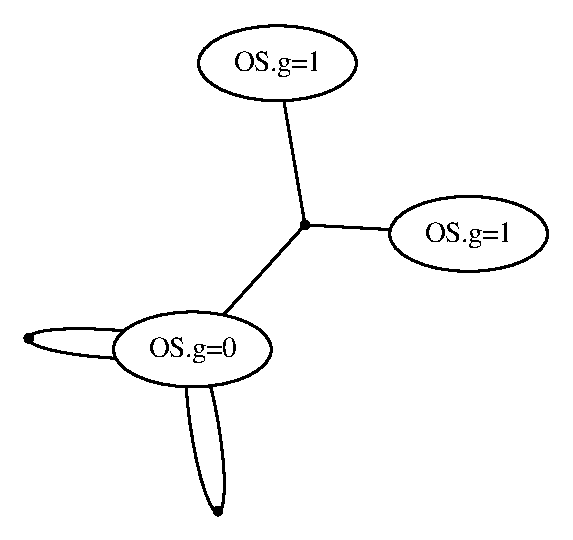
\includegraphics[width=0.3\textwidth]{figs/gluinggraph}
    \caption{Example of a gluing graph}
    \label{ch4:fig:gluinggraph}
\end{figure}

\begin{table}[h]\centering
\begin{tabular}{lp{7cm}}
    \textbf{module} & \textbf{types and functions}
    \\[4pt]
    SimplicialComplex & \ensuremath{\Conid{Vertex}}, \ensuremath{\Conid{Simplex}}, \ensuremath{\Conid{Complex}},          \newline
                        \ensuremath{\Varid{connectedComponents}}, \ensuremath{\Varid{dfsSimplices}},   \newline
                        \ensuremath{\Varid{parentSimplices}}
    \\[3pt]
    TwoDimPseudoManifold & \ensuremath{\Varid{baseSurfaces}},                               \newline
                           \ensuremath{\Varid{fixSingularity}} etc., \ensuremath{\Varid{fixAllSingularities}}, \newline
                           \ensuremath{\Varid{starSummands}} etc.
    \\[3pt]
    TwoDimManifold & \ensuremath{\Varid{identifySurface}}
    \\[3pt]
    Surface & \ensuremath{\Conid{Surface}}
    \\[3pt]
    TwoDimPseudoManifold.GluingGraph \quad & \ensuremath{\Conid{GluedD}} etc.,           \newline
                                             \ensuremath{\Varid{gluingGraph}} etc.       \newline
                                             \ensuremath{\Varid{gluingGraphSurf}} etc.
    \\[3pt]
    TwoDimPseudoManifold.GraphViz & \ensuremath{\Varid{writeGluingGraph}}, \ensuremath{\Varid{visualizeGluingGraph}}
\end{tabular}
\caption{Correspondence between presented functions and modules}
\label{ch4:tab:funcs1}
\end{table}



\section{Loop Agreement Tasks on 2-dimensional Pseudomanifolds}
\label{ch4:sec:loopspmfd}
Lastly, we consider loop agreement tasks on finite weak $2$-pseudomanifolds.
We show that the \emph{word problem} for fundamental groups of such $2$-pseudomanifolds
is solvable and use this fact in conjunction with \cref{ch3:classification}
to formulate a result about loop agreement tasks.

It is well known that the word problem for fundamental groups of closed surfaces
is solved by \emph{Dehn's Algorithm}, see
Stillwell~\cite[Sec.~6.1]{bookc:stillwell93}.
Then the following proposition is a consequence of this fact and
\cref{ch4:pmfdclass}.

\begin{thProposition}[solvability of the word problem for %
                      finite weak $2$-pseudomanifold]
    \label{ch4:wordproblem}
    %
    The word problem for the fundamental group of a $2$-dimensional finite weak
    pseudomanifold is solvable.
\end{thProposition}

\begin{proofsketch}
    First, observe that for finite weak $2$-pseudomanifolds $K,K'$ and vertices
    $v,v'$ of $K$ and $K'$, respectively, we have 
    \[  \pi_1\bigl( (K,v) \topowedge (K',v') \bigr)
            \cong \pi_1(K,v) \ast \pi_1(K',v')
    \]
    by the Seifert-van-Kampen theorem (where the wedge of complexes is defined
    in the obvious way). Secondly, let $K$ be a finite weak $2$-pseudomanifold
    and let $K'$ be the resulting complex after identifying two distinct vertices
    $v_1,v_2$ of $K$ to a single vertex~$v'$. Then we have
    \[ \pi_1(K',v') \cong \pi_1(K,v_1) \ast \Z , \]
    as can be seen by using the standard construction of the fundamental group
    of a simplicial complex in terms of generators and relations (see e.\,g.
    Herlihy~et~al.~\cite[Subsec.~15.1.2]{bookc:herlihyetal13}
    for the latter).

    Now let $K$ be a finite weak $2$-pseudomanifold and let $v\in V(K)$.
    By \cref{ch4:pmfdclass} and an inductive application of the above arguments
    we see that $\pi_1(K,v)$ is isomorphic to a free product of the form
    \[ \pi_1(S_1,x_1) \ast \cdots \ast \pi_1(S_k,x_k)
        \ast \underbrace{\Z \ast \cdots \ast \Z}_{\ell\text{ times}}
    \]
    where $S_1,\dots,S_k$ are the closed surfaces of \cref{ch4:pmfdclass},
    $s_j\in S_j$ for all $j\in\setOneto k$, and $\ell\in\N$.
    A reduced word $x_1x_2\dots x_r$ in such a free product is the identity
    element if and only if each $x_j$ is the idendity element in its corresponding group.
    Since we know how to solve the word problem for each free factor
    of~$\pi_1(K,v)$, we also know how to solve it for $\pi_1(K,v)$ itself.
    \\
\end{proofsketch}

\begin{thCorollary}[loop agreement tasks on finite weak 2-pseudomanifolds]
    Let $K,L$ be finite weak $2$-pseudomanifolds and let $\kappa,\lambda$
    be triangle loops in $K$ and $L$, respectively.
    \begin{itemize}
        \item 
            It is decidable whether $\gamma_\kappa$ or $\gamma_\lambda$
            are (pointed) contractible in $\geom{K}$ and $\geom{L}$,
            respectively.
            
        \item
            Let $\gamma_\kappa$ be (pointed) contractible. Then
            it is decidable whether $\Loop{K,\kappa}$ implements $\Loop{L,\lambda}$.
    \end{itemize}
\end{thCorollary}

\begin{proof}
    The first part is immediate from \cref{ch4:wordproblem}. For the second
    part note that the algebraic signature of~$\Loop{K,\kappa}$ is
    \[ (\pi_1(K,\dot\kappa), 1) \]
    (where $1\in\pi_1(K,\dot\kappa)$ denotes the identity element).
    Then \cref{ch3:classification}, the fact that $1$ must be mapped to the
    identity element of~$\pi_1(L,\dot\lambda)$ by any group homomorphism
    $\pi_1(K,\dot\kappa)\to\pi_1(L,\dot\lambda)$, and the first part imply
    the assertion.
    \\
\end{proof}
